\documentclass[border=1mm]{standalone}

\usepackage[dvipsnames]{xcolor}
\usepackage{tikz}
\usetikzlibrary{positioning}

\usepackage[dvipsnames]{xcolor}
\usepackage{hyperref}

\colorlet{myblue}{RoyalBlue}
\colorlet{myred}{WildStrawberry}
\colorlet{myorange}{Melon}
\colorlet{mygreen}{OliveGreen}
\colorlet{myviolet}{RoyalPurple}
\colorlet{myyellow}{Goldenrod}
\hypersetup{urlbordercolor=Green, linkbordercolor=Blue}
\darktheme

\begin{document}
	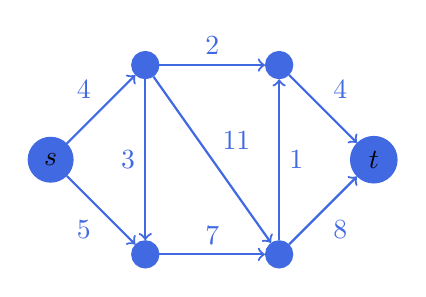
\begin{tikzpicture}[node distance={17mm}, thick, main/.style = {draw, circle, fill},
		b/.style = {myblue}]
		\node[main] (1) [b] {\textcolor{black}{$s$}};
		\node[main] (2) [above right of=1] [b] {};
		\node[main] (3) [below right of=1] [b] {};
		\node[main] (4) [right of=2] [b] {};
		\node[main] (5) [right of=3] [b] {};
		\node[main] (6) [below right of=4] [b] {\textcolor{black}{$t$}};
		\draw[->] (1) -- (2) [b] node[midway, above left] {4};
		\draw[->] (1) -- (3) [b] node[midway, below left] {5};
		\draw[->] (2) -- (3) [b] node[midway, left] {3};
		\draw[->] (3) -- (5) [b] node[midway, above] {7};
		\draw[->] (2) -- (5) [b] node[midway, above right] {11};
		\draw[->] (2) -- (4) [b] node[midway, above] {2};
		\draw[->] (5) -- (4) [b] node[midway, right] {1};
		\draw[->] (4) -- (6) [b] node[midway, above right] {4};
		\draw[->] (5) -- (6) [b] node[midway, below right] {8};
	\end{tikzpicture}
\end{document}